\documentclass[a4paper,11pt]{article}
\usepackage{amsmath, amssymb}
\usepackage{listings}
\usepackage{color}
\usepackage{hyperref}
\usepackage{geometry}
\usepackage{graphicx}
\usepackage{xcolor}
\hypersetup{
    colorlinks,
    linkcolor={red!50!black},
    citecolor={blue!50!black},
    urlcolor={blue!80!black}
}
\geometry{margin=1in}

\definecolor{codegray}{rgb}{0.5,0.5,0.5}
\definecolor{codepurple}{rgb}{0.58,0,0.82}
\definecolor{backcolour}{rgb}{0.95,0.95,0.92}

\lstdefinestyle{mystyle}{
    backgroundcolor=\color{backcolour},   
    commentstyle=\color{codegray},
    keywordstyle=\color{blue},
    numberstyle=\tiny\color{codegray},
    stringstyle=\color{codepurple},
    basicstyle=\ttfamily\footnotesize,
    breakatwhitespace=false,         
    breaklines=true,                 
    captionpos=b,                    
    keepspaces=true,                 
    numbers=left,                    
    numbersep=5pt,                  
    showspaces=false,                
    showstringspaces=false,
    showtabs=false,                  
    tabsize=2
}
\lstset{style=mystyle}

\lstdefinelanguage{PDDL}{
    keywords={define, domain, problem, :requirements, :types, :predicates, :action, :parameters, :precondition, :effect, :objects, :init, :goal, and, or, not},
    sensitive=false,
    morecomment=[l]{;},
    morestring=[b]"
}

\title{Hamiltonian Cycle Problem in PDDL \\ \large A Detailed Deliverable Package}
\author{Idriss Mortadi}
\date{}

\begin{document}

\maketitle

\tableofcontents
\newpage

\section{Introduction}
The Hamiltonian Cycle problem is a classic problem in graph theory and computer science. It involves finding a cycle in an undirected graph that visits each vertex exactly once and returns to the starting vertex. This problem is known to be NP-complete, making it a significant challenge for automated planning and optimization algorithms. In this document, we model the Hamiltonian Cycle problem using the Planning Domain Definition Language (PDDL). We provide a detailed description of the problem, our modeling choices, an illustrative example, and a sample plan to demonstrate the solution. The document is structured to guide the reader through the problem setup, the PDDL model, and the solution process.

\section{Problem Description}
The objective is to model the Hamiltonian Cycle problem using PDDL, where:
\begin{itemize}
    \item A \textbf{Hamiltonian cycle} is a cycle in an undirected graph that visits each vertex exactly once and returns to the starting vertex.
    \item The input is an undirected graph $G = (V, E)$ with a set of vertices $V$ and edges $E$.
    \item The goal is to find a cycle that visits all vertices exactly once and returns to the starting point, if such a cycle exists.
\end{itemize}
The model includes three main actions:
\begin{enumerate}
    \item \textbf{Select-Start Action:} Chooses a starting vertex for the cycle.
    \item \textbf{Move-to-Next Action:} Selects the next unvisited vertex to add to the path.
    \item \textbf{Complete-Cycle Action:} Completes the cycle by returning to the starting vertex after all vertices have been visited.
\end{enumerate}

\section{Modeling Choices and High-Level Explanation}
\subsection{Type Definitions}
We define two types to represent the entities in our problem:
\begin{itemize}
    \item \texttt{vertex}: Represents the nodes in the graph.
    \item \texttt{count}: Represents counters to track the path length.
\end{itemize}

\subsection{Predicates}
The following predicates capture the graph structure and the state of the search:
\begin{itemize}
    \item \texttt{(connected ?v1 ?v2 - vertex)}: Indicates there is an edge between vertices v1 and v2.
    \item \texttt{(visited ?v - vertex)}: Indicates vertex v has been included in the cycle.
    \item \texttt{(current ?v - vertex)}: Indicates the current position in the path construction.
    \item \texttt{(start ?v - vertex)}: Indicates the starting vertex of the cycle.
    \item \texttt{(path-length ?n - count)}: Tracks the number of vertices visited.
    \item \texttt{(next ?n1 ?n2 - count)}: Defines the successor relation for counts.
    \item \texttt{(total-vertices ?n - count)}: Stores the total number of vertices in the graph.
\end{itemize}

\subsection{Actions}
\paragraph{Select-Start Action:}  
This action selects the starting vertex for the Hamiltonian cycle. Its parameters include the vertex to select and count objects to track path length. The preconditions ensure that:
\begin{itemize}
    \item No start vertex has been selected yet.
    \item The path length is zero.
\end{itemize}
Its effects establish the starting vertex, mark it as visited, and set the path length to one.

\paragraph{Move-to-Next Action:}  
This action extends the path by moving from the current vertex to a connected, unvisited vertex. Its parameters include the current vertex, the next vertex to visit, and count objects. The preconditions ensure that:
\begin{itemize}
    \item The agent is at the "from" vertex.
    \item There is an edge connecting the "from" and "to" vertices.
    \item The "to" vertex has not been visited yet.
    \item The path length is tracked correctly.
\end{itemize}
Its effects update the current position, mark the new vertex as visited, and increment the path length.

\paragraph{Complete-Cycle Action:}  
This action completes the Hamiltonian cycle by connecting the last vertex back to the starting vertex. Its parameters include the last vertex, the first vertex, and the path length. The preconditions ensure that:
\begin{itemize}
    \item The agent is at the last vertex.
    \item There is an edge connecting the last vertex to the first vertex.
    \item All vertices have been visited (path length equals total number of vertices).
\end{itemize}
Its effects move the current position back to the starting vertex, completing the cycle.

\section{Illustrative Instance}
The following is an example instance from our implementation:

\subsection{Instance Setup}
\begin{itemize}
    \item The example uses a graph with 5 vertices, labeled v1 through v5.
    \item Edges are created with a probability of 0.4, ensuring the graph is connected.
    \item The graph is represented as an undirected graph, so each connection is bidirectional.
    \item Count objects n0 through n5 are used to track the path length.
\end{itemize}

\begin{figure}[htbp]
    \centering
    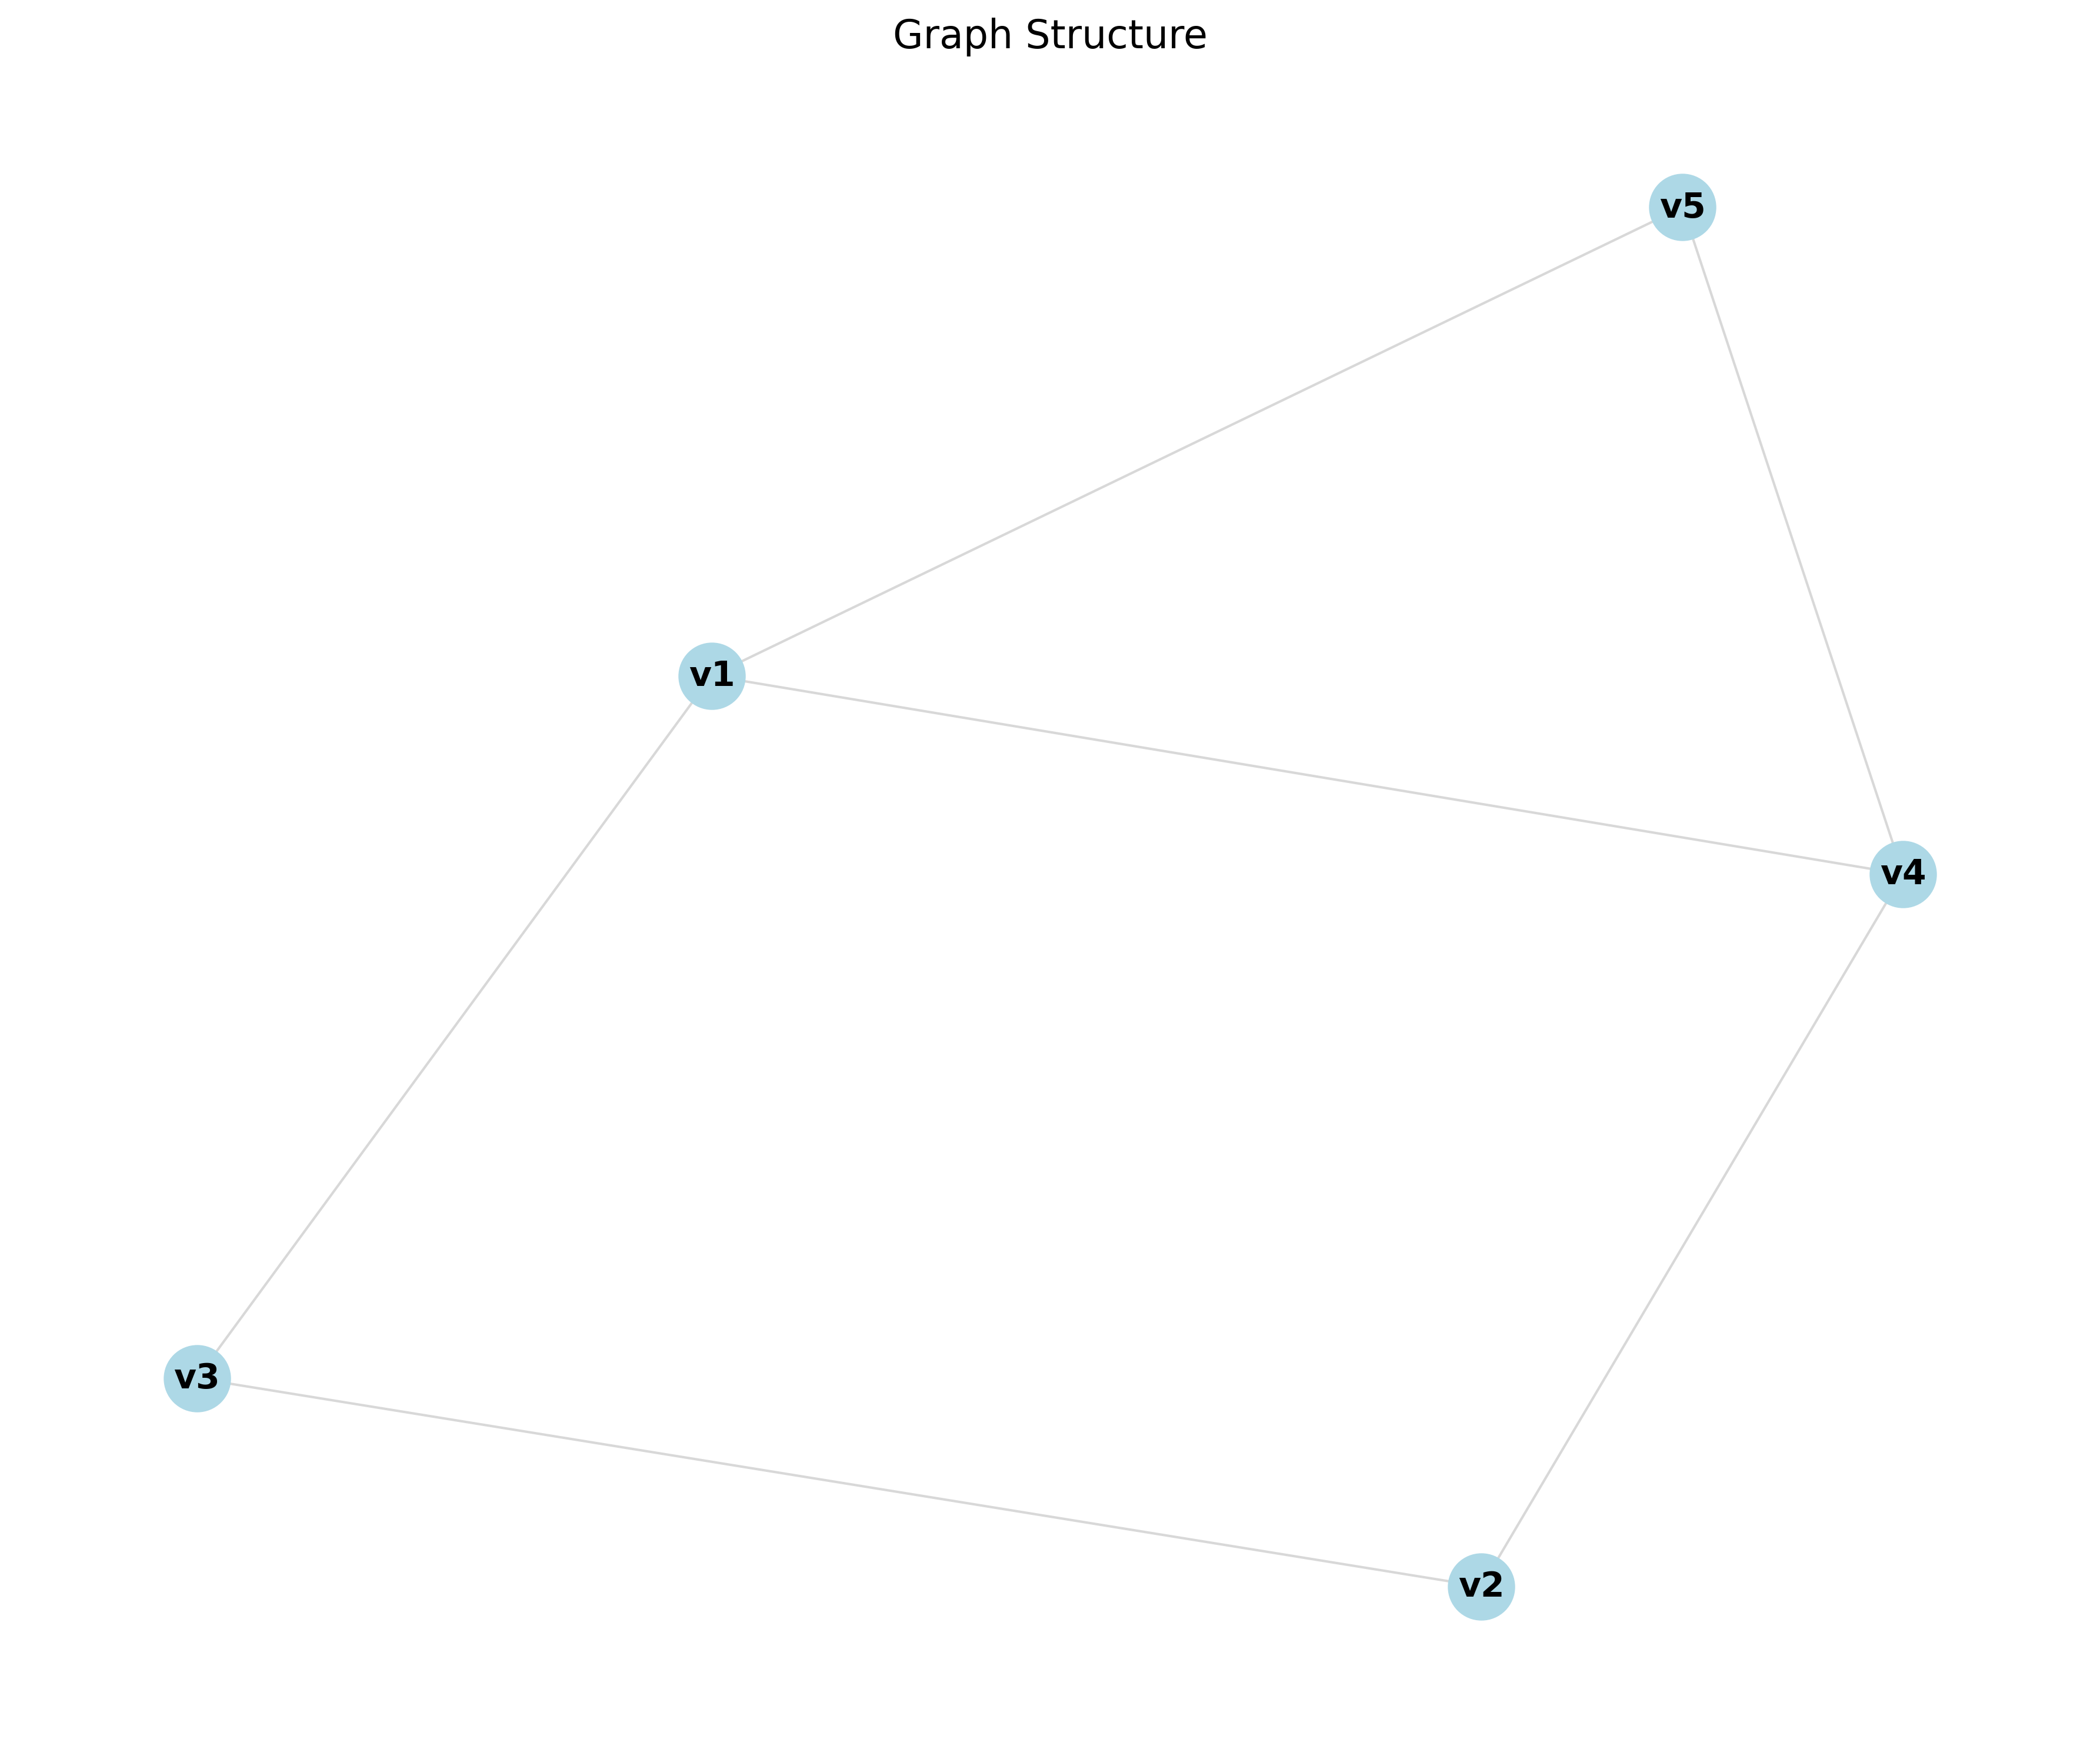
\includegraphics[width=0.8\textwidth]{../hamiltonian_cycle/problem-small_original.png}
    \caption{The original graph structure before finding a Hamiltonian cycle. Vertices are labeled v1 through v5, and edges represent valid connections between vertices.}
    \label{fig:original_graph}
\end{figure}

\subsection{Step-by-Step Example}
Let's consider a small part of the execution for illustration:
\begin{enumerate}
    \item \textbf{Initial Configuration:}
    \begin{itemize}
        \item All vertices are unvisited.
        \item No starting vertex is selected.
        \item Path length is zero.
    \end{itemize}
    \item \textbf{Step 1:}  
    Execute \texttt{select-start} action with parameters:
    \begin{center}
        \texttt{(select-start v5 n0 n1)}
    \end{center}
    Effects:
    \begin{itemize}
        \item v5 becomes the starting vertex.
        \item v5 is marked as visited.
        \item Current position is set to v5.
        \item Path length becomes 1.
    \end{itemize}
    \item \textbf{Step 2:}  
    Execute \texttt{move-to-next} action:
    \begin{center}
        \texttt{(move-to-next v5 v4 n1 n2)}
    \end{center}
    Effects:
    \begin{itemize}
        \item Current position moves from v5 to v4.
        \item v4 is marked as visited.
        \item Path length becomes 2.
    \end{itemize}
    \item \textbf{Continuing Steps:}  
    The process continues, with each step selecting an unvisited vertex adjacent to the current one and extending the path.
    \item \textbf{Final Step:}  
    After all vertices have been visited (path length is 5), execute \texttt{complete-cycle} action:
    \begin{center}
        \texttt{(complete-cycle v1 v5 n5)}
    \end{center}
    This connects the last vertex (v1) back to the starting vertex (v5), completing the Hamiltonian cycle.
\end{enumerate}

\begin{figure}[htbp]
    \centering
    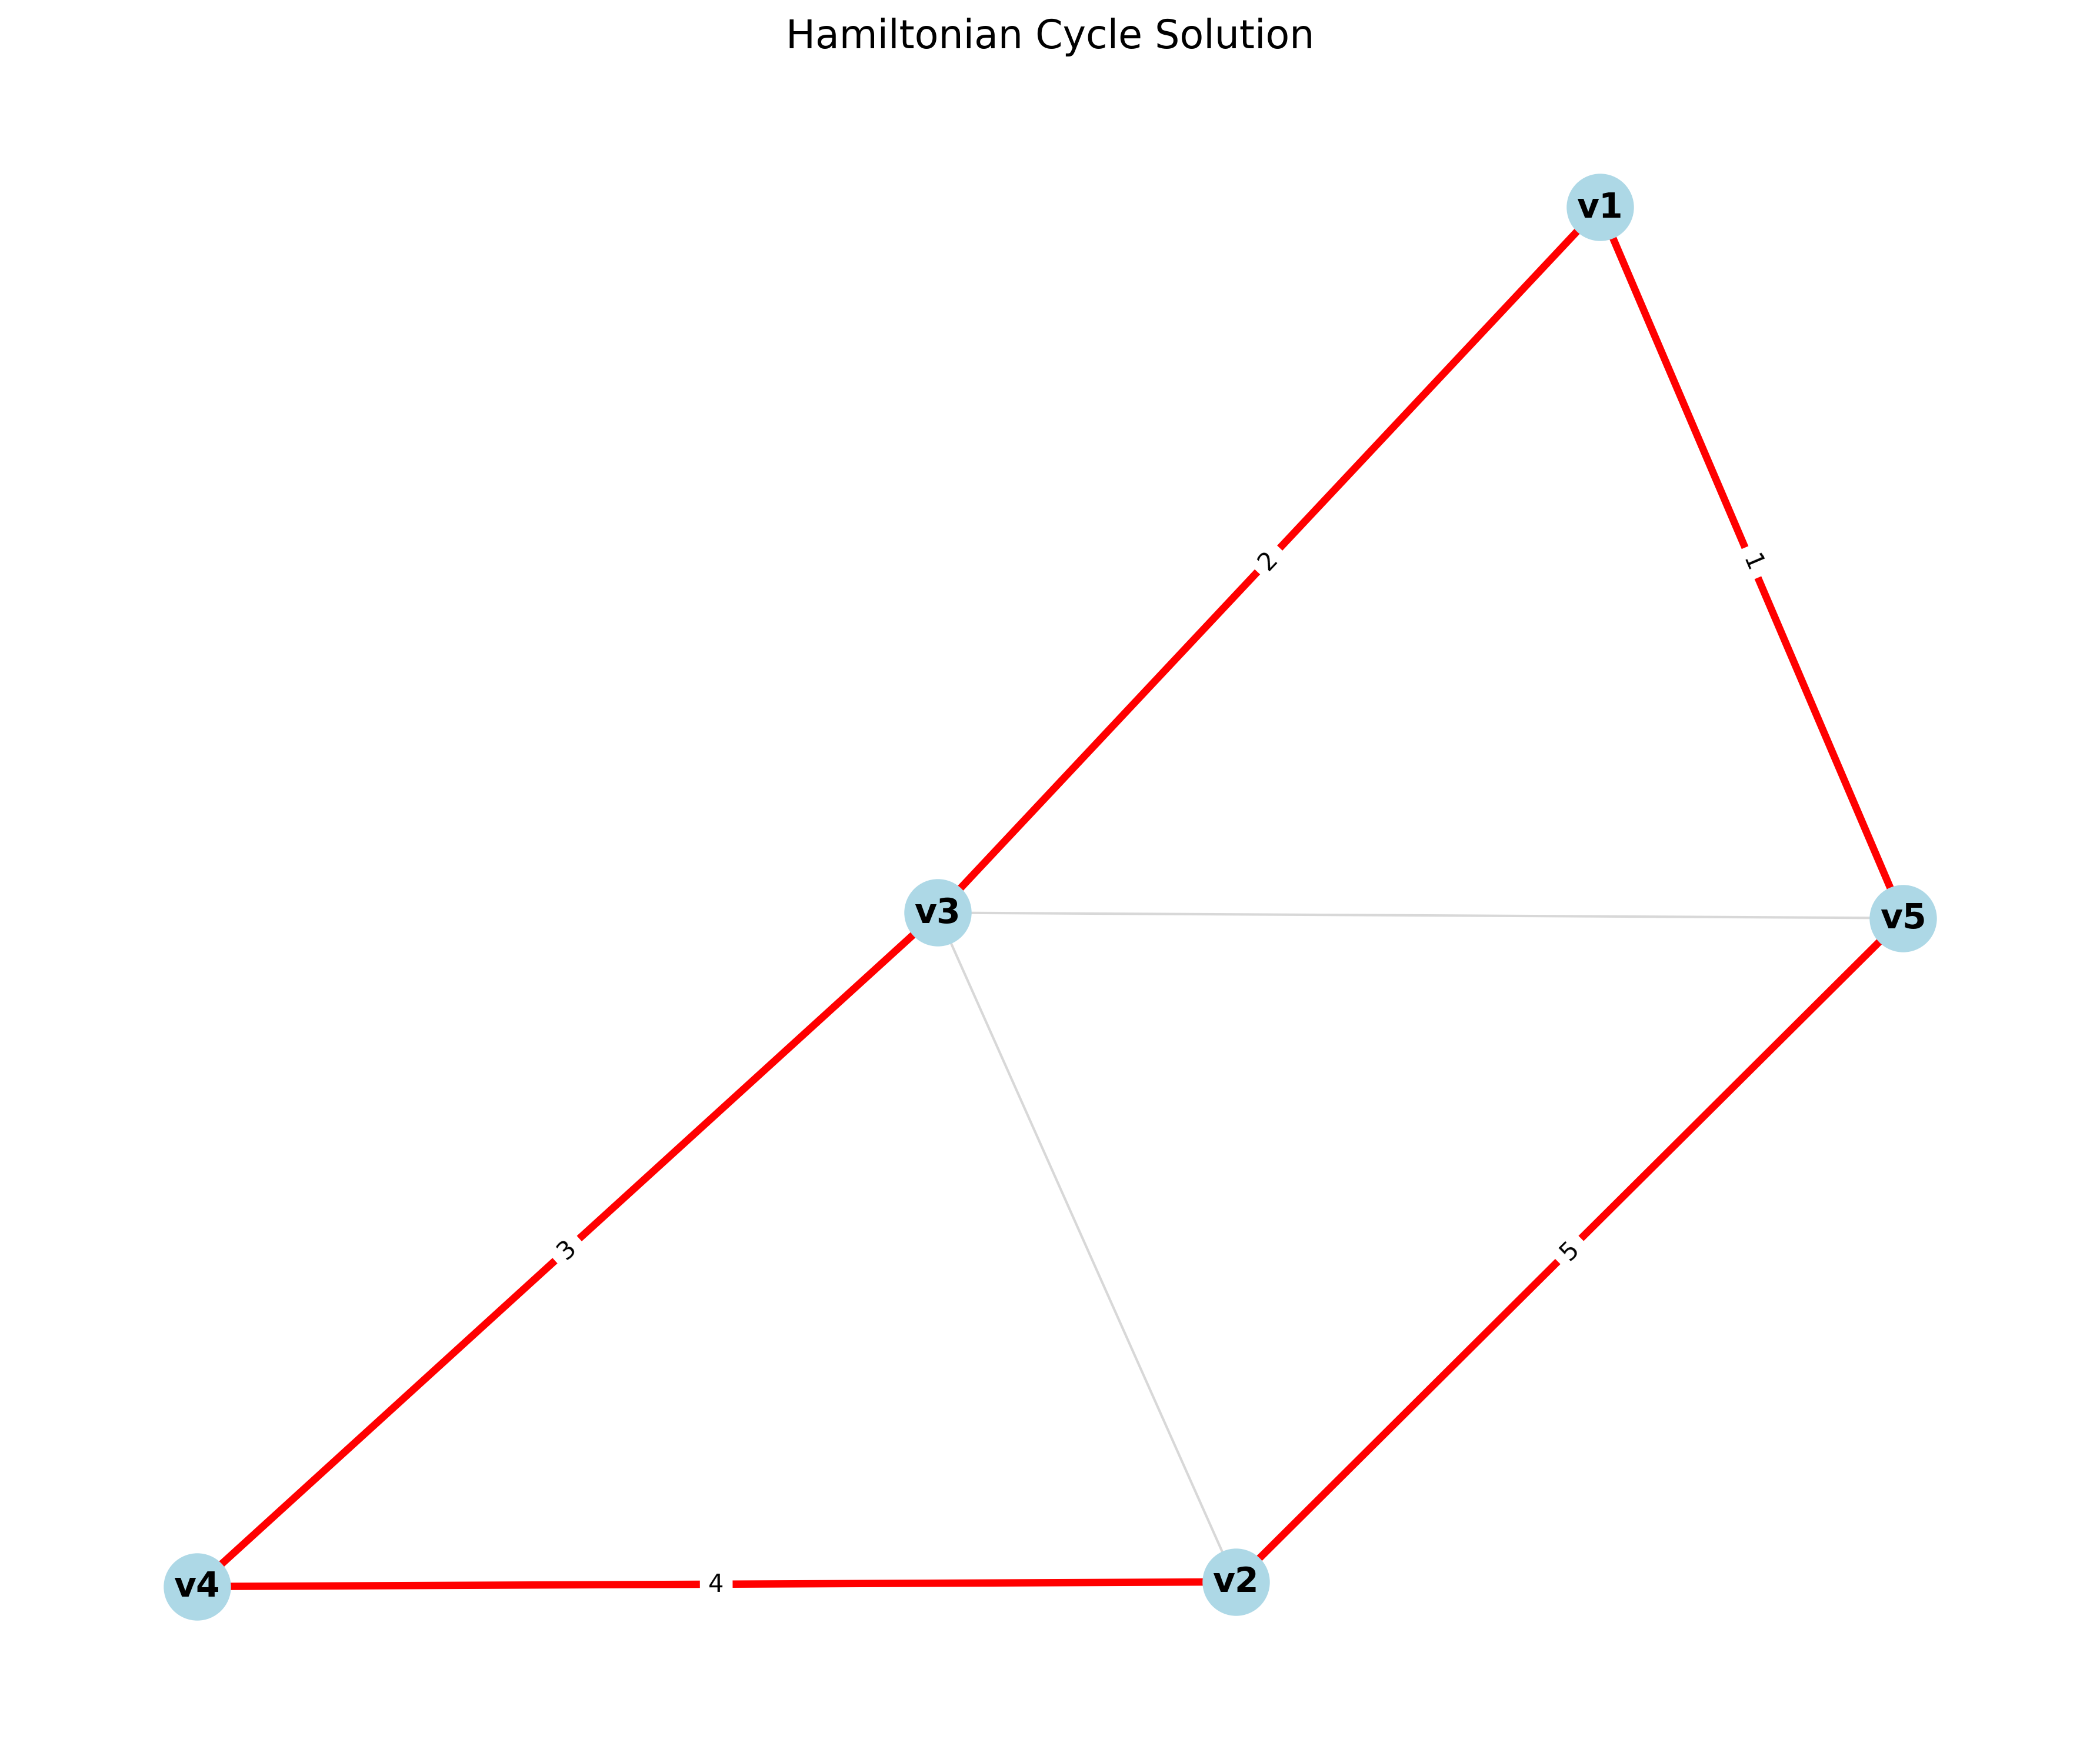
\includegraphics[width=0.8\textwidth]{../hamiltonian_cycle/problem-small_solution.png}
    \caption{The graph with the computed Hamiltonian cycle solution highlighted in red. The numbers on the edges indicate the order in which vertices are visited in the cycle.}
    \label{fig:graph_solution}
\end{figure}

\section{Sample Plan}
The following is a sample plan for the Hamiltonian Cycle problem instance described above:
\begin{center}
( select-start v5 n0 n1 )\\
( move-to-next v5 v4 n1 n2 )\\
( move-to-next v4 v2 n2 n3 )\\
( move-to-next v2 v3 n3 n4 )\\
( move-to-next v3 v1 n4 n5 )\\
( complete-cycle v1 v5 n5 )\\
( reach-goal )
\end{center}

\section{Justification and Challenges}
\subsection{Why This Problem Is Interesting}
\begin{itemize}
    \item \textbf{NP-Completeness:} The Hamiltonian cycle problem is NP-complete, making it an excellent test case for evaluating planning algorithms' ability to handle computationally challenging problems.
    \item \textbf{Real-World Applications:} The problem has applications in logistics, circuit design, and network routing, making it practically relevant.
    \item \textbf{Search Space Complexity:} The problem exemplifies the combinatorial explosion that planners face, as the number of possible paths grows factorially with the number of vertices.
\end{itemize}

\subsection{Challenges Posed by the Problem}
\begin{itemize}
    \item \textbf{Exponential Solution Space:} For a graph with n vertices, there are potentially (n-1)! different cycles to consider, creating a vast search space for the planner.
    \item \textbf{Graph Connectivity:} The solution depends critically on the graph's structure, requiring careful consideration of edge connectivity.
    \item \textbf{Performance Scaling:} As the number of vertices increases, the planner's performance can degrade rapidly, testing the limits of current planning algorithms.
\end{itemize}

\section{Graph Generation Script}
We provide a Python script that generates random connected graphs and creates corresponding PDDL problem files. The script uses NetworkX for graph generation and Matplotlib for visualization. To use the script, run:
\begin{verbatim}
python hamiltonian_cycle.py --vertices <num_vertices> --edge-prob <probability>
\end{verbatim}
This will generate a graph, create a PDDL problem file, solve the problem, and create visualizations of the original graph and the solution.

\subsection*{Installation}
To install the required Python packages, run:
\begin{verbatim}
pip install networkx matplotlib planutils
\end{verbatim}

\subsection*{FF Planner}
The script requires the FF planner to be accessible in your system's PATH. You can install the FF planner using the planutils Python package by running:
\begin{verbatim}
planutils install ff
\end{verbatim}

\end{document}
